\documentclass[tikz,border=3pt]{standalone}
\usetikzlibrary{arrows.meta}
\begin{document}
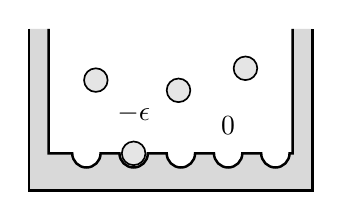
\begin{tikzpicture}[scale=1.0,>=Stealth,line width=0.9pt]
  % 容器の壁と吸着サイト（くぼみ）のある底面
  \fill[black!15] (-1.8,1.8) -- (-1.55,1.8) -- (-1.55,0.22)
    -- (-1.25,0.22) arc[start angle=180,end angle=360,radius=0.18]
    -- (-0.65,0.22) arc[start angle=180,end angle=360,radius=0.18]
    -- (-0.05,0.22) arc[start angle=180,end angle=360,radius=0.18]
    -- (0.55,0.22)  arc[start angle=180,end angle=360,radius=0.18]
    -- (1.15,0.22)  arc[start angle=180,end angle=360,radius=0.18]
    -- (1.55,0.22) -- (1.55,1.8) -- (1.8,1.8) -- (1.8,-0.25) -- (-1.8,-0.25) -- cycle;

  \draw (-1.8,1.8) -- (-1.8,-0.25) -- (1.8,-0.25) -- (1.8,1.8);
  \draw (-1.55,1.8) -- (-1.55,0.22)
    -- (-1.25,0.22) arc[start angle=180,end angle=360,radius=0.18]
    -- (-0.65,0.22) arc[start angle=180,end angle=360,radius=0.18]
    -- (-0.05,0.22) arc[start angle=180,end angle=360,radius=0.18]
    -- (0.55,0.22)  arc[start angle=180,end angle=360,radius=0.18]
    -- (1.15,0.22)  arc[start angle=180,end angle=360,radius=0.18]
    -- (1.55,0.22) -- (1.55,1.8);

  % 空間内の気体分子
  \draw[fill=black!10,line width=0.6pt] (-0.95,1.15) circle (0.15);
  \draw[fill=black!10,line width=0.6pt] (0.10,1.02) circle (0.15);
  \draw[fill=black!10,line width=0.6pt] (0.95,1.30) circle (0.15);

  % 吸着された気体分子（2番目のサイト）
  \draw[fill=black!10,line width=0.6pt] (-0.47,0.22) circle (0.15);
  \node[above,yshift=3pt] at (-0.47,0.37) {$-\epsilon$};

  % 空のサイト（4番目のサイト）
  \node[above,yshift=3pt] at (0.73,0.22) {$0$};
\end{tikzpicture}
\end{document}
